\subsection{System architecture}
A n-tier architecture is well-suited for a WMS due to its scalability, maintainability, security, and flexibility. It allows you to scale different parts of the system independently, make it easier to maintain and update the different layers, improve the security of the system, and give you more flexibility to choose different technologies or frameworks for each layer. \cite{wang2012ntier}
    \begin{figure}[!ht]
        \centering
        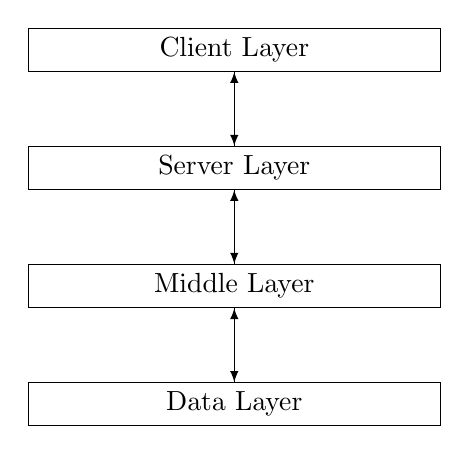
\begin{tikzpicture}[node distance=1.5cm]
            \node (client) [draw, text width=5cm, align=center] 
            {Client Layer};
            \node (server) [draw, text width=5cm, align=center, below of=client] 
            {Server Layer};
            \node (middle) [draw, text width=5cm, align=center, below of=server] 
            {Middle Layer};
            \node (data) [draw, text width=5cm, align=center, below of=middle] 
            {Data Layer};
        
            \draw [-latex] (client) -- (server);
            \draw [-latex] (server) -- (middle);
            \draw [-latex] (middle) -- (data);
            
            \draw [-latex] (server) -- (client);
            \draw [-latex] (middle) -- (server);
            \draw [-latex] (data) -- (middle);
        \end{tikzpicture}
        \caption{4-tier architecture}
        \label{fig:4-tier architecture}
    \end{figure}

\subsection{System flow}

\subsubsection{User login}

    \begin{figure}[!ht]
        \centering
        \resizebox{1\textwidth}{!}{
        \begin{sequencediagram}
            \newinst[2]{client}{Client Layer}
            \newinst[2]{server}{Server Layer}
            \newinst[2]{middle}{Middle Layer}
            \newinst[2]{data}{Data Layer}
                
            \begin{sdblock}{User login}
            {}
                \begin{call}
                    {client}{account, password}
                    {server}{access response}
                    \begin{call}
                        {server}{validate user}
                        {middle}{session response}
                        \begin{call}
                            {middle}{validation()}
                            {middle}{session response}
                            \postlevel
                            \begin{call}
                                {middle}{req account db}
                                {data}{role}
                            \end{call}
                            \postlevel
                        \end{call}
                    \end{call}
                \end{call}
            \end{sdblock}
        \end{sequencediagram}
        }
        \caption{Login sequence diagram}
        \label{fig:Login sequence diagram}
    \end{figure}
    
The sequence diagram \autoref{fig:Login sequence diagram} shows the process of a user logging into a system with different layers of the architecture interacting with each other. The sequence starts with the user entering their account and password information in the Client Layer. The Client Layer sends this information to the Server Layer, which validates the user's credentials and sends an access response. The Server Layer then sends a validation request to the Middle Layer, which retrieves the user's role from the Data Layer and performs a validation process to ensure that the user has the necessary permissions to access the requested resources. Once the validation is complete, the Middle Layer sends a session response to the Server Layer, which in turn sends the response to the Client Layer indicating that the user is authenticated and can access the system.

\subsubsection{Receiving and put-away}

    \begin{figure}[!ht]
        \centering
        \resizebox{1\textwidth}{!}{
        \begin{sequencediagram}
            \newinst[2]{client}{Client Layer}
            \newinst[2]{server}{Server Layer}
            \newinst[2]{middle}{Middle Layer}
            \newinst[2]{data}{Data Layer}

            \begin{sdblock}{New carrier}
            {algorithm depicted in \autoref{fig:Receiving and put-away flowchart diagram}}
                \begin{call}
                    {client}{carrier information}
                    {server}{put-away response}
                    \begin{call}
                        {server}{process receive}
                        {middle}{coordinate}
                        \postlevel
                        \begin{call}
                            {middle}{req $I, I_{sc}$}
                            {server}{$I, I_{sc}$}
                            \postlevel
                        \end{call}
                        \begin{call}
                            {middle}{algorithm \ref{ca:receiving and put-away}()}
                            {middle}{coordinate}
                            \postlevel
                            \begin{call}
                                {middle}{req statistic db}
                                {data}{$X_t$}
                                \postlevel
                            \end{call}
                            \postlevel
                            \begin{call}
                                {middle}{req column db}
                                {data}{$C_c, T_c, X_c$}
                                \postlevel
                            \end{call}
                            \postlevel
                            \begin{call}
                                {middle}{req slot db}
                                {data}{$I_p, X_s, E_s$}
                                \postlevel
                            \end{call}
                            \postlevel
                            \begin{call}
                                {middle}{send $E_s, I_{sc}, T_s$}
                                {data}{slot db res}
                                \postlevel
                            \end{call}
                            \postlevel
                        \end{call}
                    \end{call}
                \end{call}
            \end{sdblock}
            
        \end{sequencediagram}
        }
        \caption{Receiving and put-away sequence diagram}
        \label{fig:Receiving and put-away sequence diagram}
    \end{figure}
    
The sequence diagram \autoref{fig:Receiving and put-away sequence diagram} depicts the process of adding a new carrier to a WMS. The sequence starts with the Client Layer sending carrier information to the Server Layer. The Server Layer processes the request by calling the "receive" function in the Middle Layer. The Middle Layer coordinates the request and calls the "receiving and put-away" algorithm, which updates the databases with the new carrier information and sends a coordinate back to the Server Layer. The Server Layer then sends a put-away response to the Client Layer indicating that the carrier has been successfully integrated to the system.

\subsubsection{Order fulfillment}

    \begin{figure}[!ht]
        \centering
        \resizebox{1\textwidth}{!}{
        \begin{sequencediagram}
            \newinst[2]{client}{Client Layer}
            \newinst[2]{server}{Server Layer}
            \newinst[2]{middle}{Middle Layer}
            \newinst[2]{data}{Data Layer}
             
            \begin{sdblock}{New order}
            {algorithm depicted in \autoref{fig:Order fulfillment flowchart diagram}}
                \begin{call}
                    {client}{order information}
                    {server}{picking response}
                    \begin{call}
                        {server}{process order}
                        {middle}{coordinate, date}
                        \postlevel
                        \begin{call}
                            {middle}{req $I(i), n(i), I_d$}
                            {server}{$I(i), n(i), I_d$}
                            \postlevel
                        \end{call}
                        \begin{call}
                            {middle}{algorithm \ref{ca:order fulfillment}()}
                            {middle}{coordinate, date}
                            \postlevel
                            \begin{call}
                                {middle}{req statistic db}
                                {data}{$Q_a, X_o$}
                                \postlevel
                            \end{call}
                            \postlevel
                            \begin{call}
                                {middle}{$EMC()$}
                                {middle}{date}
                                \postlevel
                                \begin{call}
                                    {middle}{req emc db}
                                    {data}{$EMC$}
                                    \postlevel
                                \end{call}
                                \postlevel
                            \end{call}
                            \postlevel
                            \begin{call}
                                {middle}{req column db}
                                {data}{$C_c, T_c, X_c$}
                                \postlevel
                            \end{call}
                            \postlevel
                            \begin{call}
                                {middle}{req slot db}
                                {data}{$X_s, E_s$}
                                \postlevel
                            \end{call}
                            \postlevel
                            \begin{call}
                                {middle}{send $R_d, I_d, T_d$}
                                {data}{slot db res}
                                \postlevel
                            \end{call}
                            \postlevel
                        \end{call}
                    \end{call}
                \end{call}
            \end{sdblock}
            
        \end{sequencediagram}
        }
        \caption{Order fulfillment sequence diagram}
        \label{fig:Order fulfillment sequence diagram}
    \end{figure}
    
The sequence diagram \autoref{fig:Order fulfillment sequence diagram} shows the process of fulfilling a new order in a warehouse management system. The sequence starts with the Client Layer sending order information to the Server Layer. The Server Layer processes the request by calling the "order" function in the Middle Layer. The Middle Layer coordinates the request and calls the "order fulfillment" algorithm, which updates the databases with the order information and sends a coordinate and date response back to the Server. The Server then sends a picking response to the Client Layer indicating that the order can be fulfilled.

\subsubsection{Daily replenishment}

    \begin{figure}[!ht]
        \centering
        \resizebox{1\textwidth}{!}{
        \begin{sequencediagram}
            \newinst[2]{client}{Client Layer}
            \newinst[2]{server}{Server Layer}
            \newinst[2]{middle}{Middle Layer}
            \newinst[2]{data}{Data Layer}
                
            \begin{sdblock}{Daily replenishment}
            {algorithm depicted in \autoref{fig:Daily replenishment sequence diagram}}
                \begin{call}
                    {server}{cycle counter}
                    {middle}{cycle conclude}
                    \begin{call}
                        {middle}{algorithm \ref{ca:replenishment}()}
                        {middle}{replenish response}
                        \postlevel
                        \begin{call}
                            {middle}{req parameter db}
                            {data}{$S_a$}
                            \postlevel
                        \end{call}
                        \postlevel
                        \begin{call}
                            {middle}{req slot db}
                            {data}{$E_s$}
                            \postlevel
                        \end{call}
                        \postlevel
                        \begin{call}
                            {middle}{req product db}
                            {data}{$B$}
                            \postlevel
                        \end{call}
                        \postlevel
                        \begin{call}
                            {middle}{req record db}
                            {data}{$g_r, G_r, H_r$}
                            \postlevel
                        \end{call}
                        \begin{call}
                            {middle}{factory request}
                            {server}{factory response}
                            \begin{call}
                                {server}{factory request}
                                {client}{factory response}
                                \postlevel
                            \end{call}
                        \end{call}
                    \end{call}
                \end{call}
            \end{sdblock}

        \end{sequencediagram}
        }
        \caption{Daily replenishment sequence diagram}
        \label{fig:Daily replenishment sequence diagram}
    \end{figure}
    
The sequence diagram \autoref{fig:Daily replenishment sequence diagram} illustrates the daily replenishment process in a warehouse management system. The sequence begins when the Server Layer sends a cycle counter to the Middle Layer, which then calls the "daily replenishment" algorithm. The algorithm interacts with several databases in the Data Layer, such as the parameter database, slot database, product database, and record database. The algorithm also sends a factory request to the Server Layer, which sends the request to the Client Layer to obtain the necessary products. Once the factory response is received, the Middle Layer send a replenish response to conclude the cycle.

\subsubsection{Space allocation}

    \begin{figure}[!ht]
        \centering
        \resizebox{1\textwidth}{!}{
        \begin{sequencediagram}
            \newinst[2]{client}{Client Layer}
            \newinst[2]{server}{Server Layer}
            \newinst[2]{middle}{Middle Layer}
            \newinst[2]{data}{Data Layer}
                
            \begin{sdblock}{Space allocation}
            {algorithm depicted in \autoref{fig:Space allocation sequence diagram}}
                \begin{call}
                    {server}{cycle counter}
                    {middle}{cycle conclude}
                    \begin{call}
                        {middle}{algorithm \ref{ca:space allocation}()}
                        {middle}{$K$}
                        \postlevel
                        \begin{call}
                            {middle}{req parameter db}
                            {data}{$S_a$}
                            \postlevel
                        \end{call}
                        \postlevel
                        \begin{call}
                            {middle}{req product db}
                            {data}{$B$}
                            \postlevel
                        \end{call}
                        \postlevel
                        \begin{call}
                            {middle}{req record db}
                            {data}{$g, G, H$}
                            \postlevel
                        \end{call}
                        \postlevel
                    \end{call}
                    \postlevel
                    \begin{call}
                        {middle}{allocate()}
                        {middle}{allocate response}
                        \postlevel
                        \begin{call}
                            {middle}{req slot db}
                            {data}{$X_s, E_s, I_s$}
                            \postlevel
                        \end{call}
                        \postlevel
                        \begin{call}
                            {middle}{req column db}
                            {data}{$X_c, C_c, I_c$}
                            \postlevel
                        \end{call}
                        \postlevel
                        \begin{call}
                            {middle}{send $X_s, I_p$}
                            {data}{slot db res}
                            \postlevel
                        \end{call}
                        \postlevel
                    \end{call}
                \end{call}
            \end{sdblock}

        \end{sequencediagram}
        }
        \caption{Space allocation sequence diagram}
        \label{fig:Space allocation sequence diagram}
    \end{figure}
    
The sequence diagram in \autoref{fig:Space allocation sequence diagram} illustrates the process of space allocation in a warehouse management system. The sequence begins with the Server Layer sending a cycle counter to the Middle Layer, which then calls the "space allocation" algorithm. The algorithm interacts with several databases in the Data Layer to output a quota for each product. The algorithm then calls the "allocate" function, using the quota to allocate space for each product. The Middle Layer then sends the allocation information to the Data Layer, which updates the slot database. Finally, the cycle concludes.

\newpage